\documentclass{standalone}
\usepackage{tikz}
\usetikzlibrary{patterns, positioning}


\begin{document}
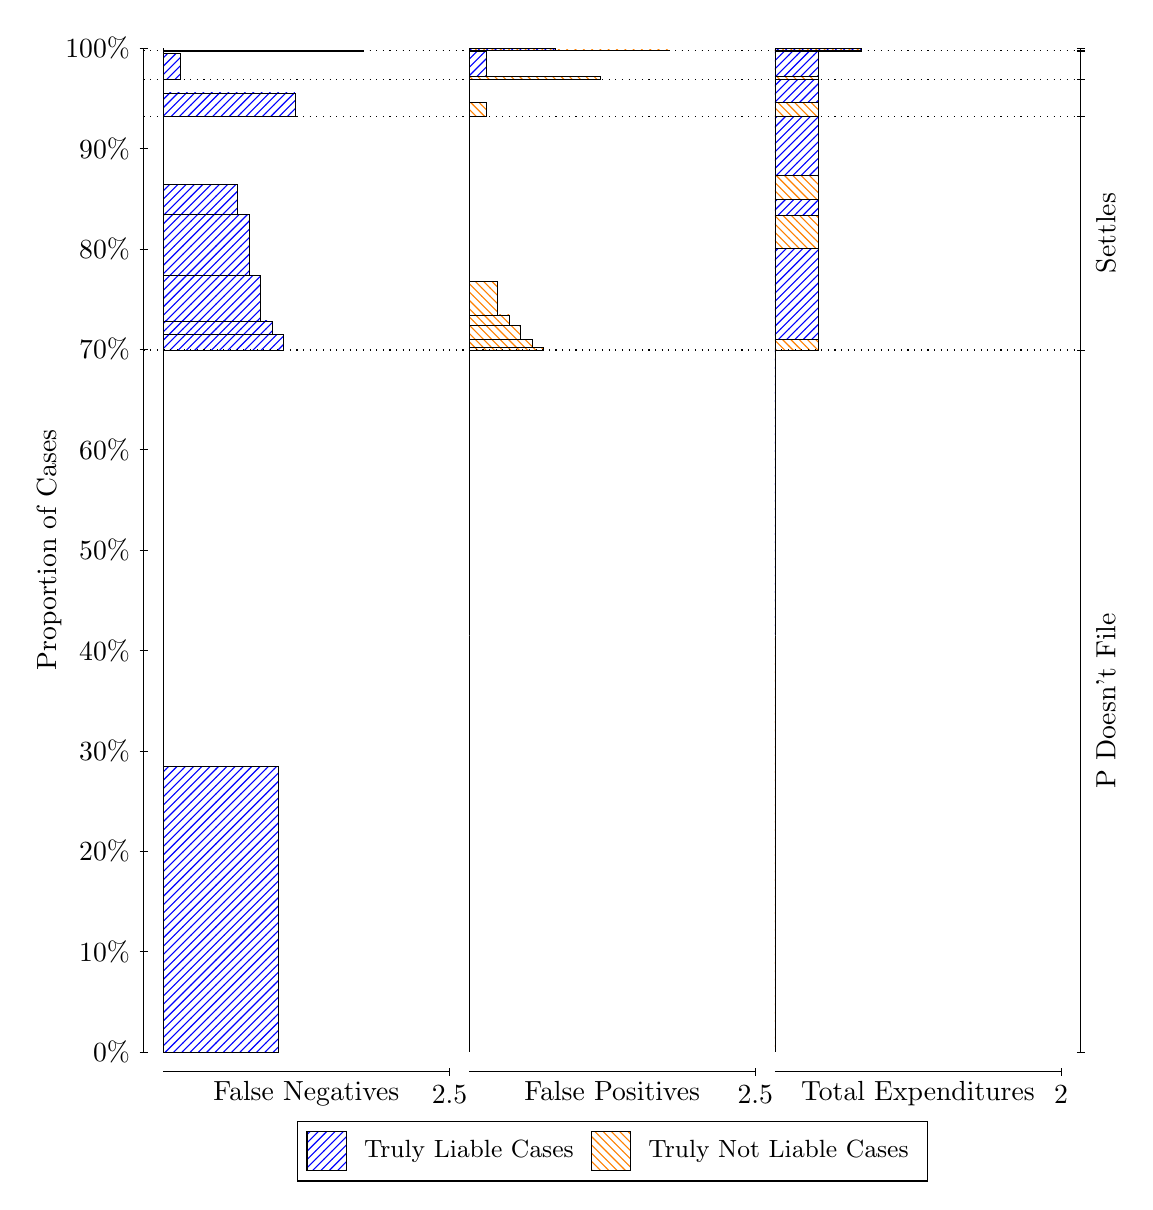
\begin{tikzpicture}
\draw[black, very thin] (1.5,1.75) -- (1.5,14.5);
\node[rotate=90, text=black, anchor=center] at (0.3, 8.125) {Proportion of Cases};
\draw[black, very thin] (1.45,1.75) -- (1.55,1.75);
\node[text=black, anchor=east] at (1.45, 1.75) {0\%};
\draw[black, very thin] (1.45,3.025) -- (1.55,3.025);
\node[text=black, anchor=east] at (1.45, 3.025) {10\%};
\draw[black, very thin] (1.45,4.3) -- (1.55,4.3);
\node[text=black, anchor=east] at (1.45, 4.3) {20\%};
\draw[black, very thin] (1.45,5.575) -- (1.55,5.575);
\node[text=black, anchor=east] at (1.45, 5.575) {30\%};
\draw[black, very thin] (1.45,6.85) -- (1.55,6.85);
\node[text=black, anchor=east] at (1.45, 6.85) {40\%};
\draw[black, very thin] (1.45,8.125) -- (1.55,8.125);
\node[text=black, anchor=east] at (1.45, 8.125) {50\%};
\draw[black, very thin] (1.45,9.4) -- (1.55,9.4);
\node[text=black, anchor=east] at (1.45, 9.4) {60\%};
\draw[black, very thin] (1.45,10.675) -- (1.55,10.675);
\node[text=black, anchor=east] at (1.45, 10.675) {70\%};
\draw[black, very thin] (1.45,11.95) -- (1.55,11.95);
\node[text=black, anchor=east] at (1.45, 11.95) {80\%};
\draw[black, very thin] (1.45,13.225) -- (1.55,13.225);
\node[text=black, anchor=east] at (1.45, 13.225) {90\%};
\draw[black, very thin] (1.45,14.5) -- (1.55,14.5);
\node[text=black, anchor=east] at (1.45, 14.5) {100\%};

\draw[black, very thin] (13.4,1.75) -- (13.4,14.5);
\draw[black, very thin] (13.35,1.75) -- (13.45,1.75);
\node[anchor=west] at (13.35, 1.75) {};
\draw[black, very thin] (13.35,10.665) -- (13.45,10.665);
\node[anchor=west] at (13.35, 10.665) {};
\draw[black, very thin] (13.35,13.635) -- (13.45,13.635);
\node[anchor=west] at (13.35, 13.635) {};
\draw[black, very thin] (13.35,14.102) -- (13.45,14.102);
\node[anchor=west] at (13.35, 14.102) {};
\draw[black, very thin] (13.35,14.463) -- (13.45,14.463);
\node[anchor=west] at (13.35, 14.463) {};
\draw[black, very thin] (13.35,14.472) -- (13.45,14.472);
\node[anchor=west] at (13.35, 14.472) {};
\draw[black, very thin] (13.35,14.5) -- (13.45,14.5);
\node[anchor=west] at (13.35, 14.5) {};

\draw[black, very thin, pattern color=blue, pattern=north east lines] (1.75,1.75) rectangle (3.2033,5.3747);
\draw[black, very thin, pattern color=orange, pattern=north west lines] (1.75,5.3747) rectangle (1.75,10.665);
\draw[black, very thin, pattern color=blue, pattern=north east lines] (1.75,10.665) rectangle (3.276,10.861);
\draw[black, very thin, pattern color=blue, pattern=north east lines] (1.75,10.861) rectangle (3.1307,11.034);
\draw[black, very thin, pattern color=blue, pattern=north east lines] (1.75,11.034) rectangle (2.9853,11.612);
\draw[black, very thin, pattern color=blue, pattern=north east lines] (1.75,11.612) rectangle (2.84,12.392);
\draw[black, very thin, pattern color=blue, pattern=north east lines] (1.75,12.392) rectangle (2.6947,12.764);
\draw[black, very thin, pattern color=orange, pattern=north west lines] (1.75,12.764) rectangle (1.75,13.635);
\draw[black, very thin, pattern color=blue, pattern=north east lines] (1.75,13.635) rectangle (3.4213,13.931);
\draw[black, very thin, pattern color=orange, pattern=north west lines] (1.75,13.931) rectangle (1.75,14.102);
\draw[black, very thin, pattern color=blue, pattern=north east lines] (1.75,14.102) rectangle (1.968,14.429);
\draw[black, very thin, pattern color=orange, pattern=north west lines] (1.75,14.429) rectangle (1.75,14.463);
\draw[black, very thin, pattern color=blue, pattern=north east lines] (1.75,14.463) rectangle (4.2933,14.468);
\draw[black, very thin, pattern color=orange, pattern=north west lines] (1.75,14.468) rectangle (1.75,14.472);
\draw[black, very thin, pattern color=orange, pattern=north west lines] (1.75,14.472) rectangle (1.75,14.477);
\draw[black, very thin, pattern color=blue, pattern=north east lines] (1.75,14.477) rectangle (1.75,14.5);
\draw[black, very thin, pattern color=orange, pattern=north west lines] (5.6333,1.75) rectangle (5.6333,7.0405);
\draw[black, very thin, pattern color=blue, pattern=north east lines] (5.6333,7.0405) rectangle (5.6333,10.665);
\draw[black, very thin, pattern color=orange, pattern=north west lines] (5.6333,10.665) rectangle (6.578,10.695);
\draw[black, very thin, pattern color=orange, pattern=north west lines] (5.6333,10.695) rectangle (6.4327,10.8);
\draw[black, very thin, pattern color=orange, pattern=north west lines] (5.6333,10.8) rectangle (6.2873,10.978);
\draw[black, very thin, pattern color=orange, pattern=north west lines] (5.6333,10.978) rectangle (6.142,11.111);
\draw[black, very thin, pattern color=orange, pattern=north west lines] (5.6333,11.111) rectangle (5.9967,11.535);
\draw[black, very thin, pattern color=blue, pattern=north east lines] (5.6333,11.535) rectangle (5.6333,13.635);
\draw[black, very thin, pattern color=orange, pattern=north west lines] (5.6333,13.635) rectangle (5.8513,13.805);
\draw[black, very thin, pattern color=blue, pattern=north east lines] (5.6333,13.805) rectangle (5.6333,14.102);
\draw[black, very thin, pattern color=orange, pattern=north west lines] (5.6333,14.102) rectangle (7.3047,14.136);
\draw[black, very thin, pattern color=blue, pattern=north east lines] (5.6333,14.136) rectangle (5.8513,14.463);
\draw[black, very thin, pattern color=orange, pattern=north west lines] (5.6333,14.463) rectangle (5.6333,14.467);
\draw[black, very thin, pattern color=blue, pattern=north east lines] (5.6333,14.467) rectangle (5.6333,14.472);
\draw[black, very thin, pattern color=orange, pattern=north west lines] (5.6333,14.472) rectangle (8.1767,14.477);
\draw[black, very thin, pattern color=blue, pattern=north east lines] (5.6333,14.477) rectangle (6.7233,14.5);
\draw[black, very thin, pattern color=orange, pattern=north west lines] (9.5167,1.75) rectangle (9.5167,7.0405);
\draw[black, very thin, pattern color=blue, pattern=north east lines] (9.5167,7.0405) rectangle (9.5167,10.665);
\draw[black, very thin, pattern color=orange, pattern=north west lines] (9.5167,10.665) rectangle (10.062,10.8);
\draw[black, very thin, pattern color=blue, pattern=north east lines] (9.5167,10.8) rectangle (10.062,11.952);
\draw[black, very thin, pattern color=orange, pattern=north west lines] (9.5167,11.952) rectangle (10.062,12.377);
\draw[black, very thin, pattern color=blue, pattern=north east lines] (9.5167,12.377) rectangle (10.062,12.573);
\draw[black, very thin, pattern color=orange, pattern=north west lines] (9.5167,12.573) rectangle (10.062,12.884);
\draw[black, very thin, pattern color=blue, pattern=north east lines] (9.5167,12.884) rectangle (10.062,13.635);
\draw[black, very thin, pattern color=orange, pattern=north west lines] (9.5167,13.635) rectangle (10.062,13.805);
\draw[black, very thin, pattern color=blue, pattern=north east lines] (9.5167,13.805) rectangle (10.062,14.102);
\draw[black, very thin, pattern color=orange, pattern=north west lines] (9.5167,14.102) rectangle (10.062,14.136);
\draw[black, very thin, pattern color=blue, pattern=north east lines] (9.5167,14.136) rectangle (10.062,14.463);
\draw[black, very thin, pattern color=orange, pattern=north west lines] (9.5167,14.463) rectangle (10.607,14.467);
\draw[black, very thin, pattern color=blue, pattern=north east lines] (9.5167,14.467) rectangle (10.607,14.472);
\draw[black, very thin, pattern color=orange, pattern=north west lines] (9.5167,14.472) rectangle (10.607,14.477);
\draw[black, very thin, pattern color=blue, pattern=north east lines] (9.5167,14.477) rectangle (10.607,14.5);
\draw[black, dotted] (1.5,10.665) -- (13.4,10.665);
\draw[black, dotted] (1.5,13.635) -- (13.4,13.635);
\draw[black, dotted] (1.5,14.102) -- (13.4,14.102);
\draw[black, dotted] (1.5,14.463) -- (13.4,14.463);
\draw[black, dotted] (1.5,14.472) -- (13.4,14.472);
\draw[black, very thin] (1.75,1.5) -- (5.3833,1.5);
\node[text=black, anchor=north] at (3.5667, 1.5) {False Negatives};
\draw[black, very thin] (5.3833,1.45) -- (5.3833,1.55);
\node[text=black, anchor=north] at (5.3833, 1.45) {2.5};

\draw[black, very thin] (5.6333,1.5) -- (9.2667,1.5);
\node[text=black, anchor=north] at (7.45, 1.5) {False Positives};
\draw[black, very thin] (9.2667,1.45) -- (9.2667,1.55);
\node[text=black, anchor=north] at (9.2667, 1.45) {2.5};

\draw[black, very thin] (9.5167,1.5) -- (13.15,1.5);
\node[text=black, anchor=north] at (11.333, 1.5) {Total Expenditures};
\draw[black, very thin] (13.15,1.45) -- (13.15,1.55);
\node[text=black, anchor=north] at (13.15, 1.45) {2};

\node[text=black, centered, rotate=90] at (13.72, 6.2076) {P Doesn't File};
\node[text=black, centered, rotate=90] at (13.72, 12.15) {Settles};





\draw (7.449999999999999,1.5) node[draw=none] (baseCoordinate) {};
\begin{scope}[align=center]
        \matrix[scale=0.5, draw=black, below=0.5cm of baseCoordinate, nodes={draw}, column sep=0.1cm]{
            \node[rectangle, draw, minimum width=0.5cm, minimum height=0.5cm, pattern color=blue, pattern=north east lines] {}; &
            \node[draw=none, font=\small, text=black] (B) {Truly Liable Cases}; &
            \node[rectangle, draw, minimum width=0.5cm, minimum height=0.5cm, pattern color=orange, pattern=north west lines] {}; &
            \node[draw=none, font=\small, text=black] (B) {Truly Not Liable Cases}; \\
            };
\end{scope}

\end{tikzpicture}
\end{document}